\documentclass[10pt]{beamer}
\usetheme{metropolis}
\usepackage{booktabs}
\usepackage{algorithm}
\usepackage{algorithmic}
\usepackage{amsmath}
\usepackage{graphicx}
\usepackage{tikz}
\usetikzlibrary{shapes,arrows,positioning}

\title{Statistical and Machine Learning Methods}
\subtitle{Stratified Sampling, Isolation Forest, and DBSCAN}
\date{\today}
\author{GOD}


\begin{document}
	
	\maketitle
	
	\begin{frame}{Table of Contents}
		\setbeamertemplate{section in toc}[sections numbered]
		\tableofcontents
	\end{frame}
	
	% ============================================
	% SECTION 1: STRATIFIED SAMPLING
	% ============================================
	\section{Stratified Sampling}
	
	\begin{frame}{Introduction to Sampling}
		\textbf{Why Sampling?}
		\begin{itemize}
			\item Population data often too large or expensive to collect
			\item Need representative subset for analysis
			\item Inference from sample to population
		\end{itemize}
		
		\vspace{0.5cm}
		\textbf{Sampling Methods:}
		\begin{itemize}
			\item Simple Random Sampling
			\item Systematic Sampling
			\item \alert{Stratified Sampling} ← Our Focus
			\item Cluster Sampling
		\end{itemize}
	\end{frame}
	
	\begin{frame}{What is Stratified Sampling?}
		\textbf{Definition:}
		A probability sampling technique where the population is divided into homogeneous subgroups (strata) and samples are drawn from each stratum.
		
		\vspace{0.5cm}
		\textbf{Key Characteristics:}
		\begin{itemize}
			\item Population divided into mutually exclusive groups
			\item Each group shares similar characteristics
			\item Random sampling within each stratum
			\item Combines samples from all strata
		\end{itemize}
		
		\vspace{0.5cm}
		\textbf{Stratification Variables:}
		Age, gender, income, education, geographic location, etc.
	\end{frame}
	
	
	
	\begin{frame}{Stratified Sampling: Visual Representation}
		\begin{center}
			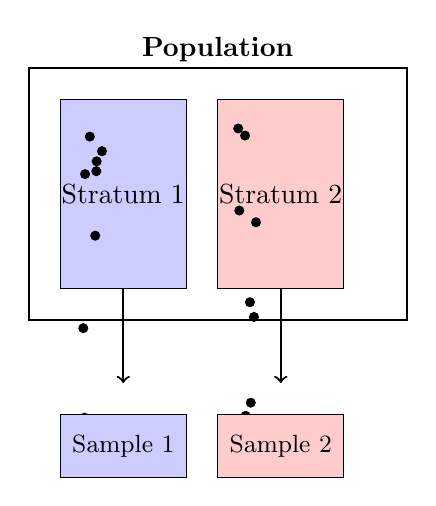
\begin{tikzpicture}[scale=0.8]
				% Population
				\draw[thick] (0,0) rectangle (6,4);
				\node at (3,4.3) {\textbf{Population}};
				
				% Stratum 1
				\draw[fill=blue!20] (0.5,0.5) rectangle (2.5,3.5);
				\node at (1.5,2) {Stratum 1};
				\foreach \i in {1,...,8} {
					\fill (1+0.2*rand,0.8+2.4*rand) circle (0.08);
				}
				
				% Stratum 2
				\draw[fill=red!20] (3,0.5) rectangle (5,3.5);
				\node at (4,2) {Stratum 2};
				\foreach \i in {1,...,8} {
					\fill (3.5+0.2*rand,0.8+2.4*rand) circle (0.08);
				}
				
				% Arrows to samples
				\draw[->,thick] (1.5,0.5) -- (1.5,-1);
				\draw[->,thick] (4,0.5) -- (4,-1);
				
				% Samples
				\draw[fill=blue!20] (0.5,-1.5) rectangle (2.5,-2.5);
				\node at (1.5,-2) {\small Sample 1};
				
				\draw[fill=red!20] (3,-1.5) rectangle (5,-2.5);
				\node at (4,-2) {\small Sample 2};
			\end{tikzpicture}
		\end{center}
	\end{frame}
	
	\begin{frame}{Types of Stratified Sampling}
		\textbf{1. Proportionate Stratified Sampling}
		\begin{itemize}
			\item Sample size from each stratum proportional to stratum size
			\item Formula: $n_i = n \times \frac{N_i}{N}$
			\item Where $n_i$ = sample from stratum $i$, $N_i$ = stratum size
		\end{itemize}
		
		\vspace{0.5cm}
		\textbf{2. Disproportionate Stratified Sampling}
		\begin{itemize}
			\item Sample sizes not proportional to stratum sizes
			\item Used when strata have different variances
			\item Optimal allocation: $n_i = n \times \frac{N_i \sigma_i}{\sum N_i \sigma_i}$
		\end{itemize}
	\end{frame}
	
	\begin{frame}{Mathematical Framework}
		\textbf{Stratified Sample Mean:}
		$$\bar{y}_{st} = \sum_{h=1}^{L} W_h \bar{y}_h$$
		
		where $W_h = \frac{N_h}{N}$ (stratum weight), $\bar{y}_h$ = sample mean in stratum $h$
		
		\vspace{0.5cm}
		\textbf{Variance of Stratified Sample Mean:}
		$$Var(\bar{y}_{st}) = \sum_{h=1}^{L} W_h^2 \frac{\sigma_h^2}{n_h} \left(1 - \frac{n_h}{N_h}\right)$$
		
		\vspace{0.5cm}
		\textbf{Standard Error:}
		$$SE(\bar{y}_{st}) = \sqrt{Var(\bar{y}_{st})}$$
	\end{frame}
	
	\begin{frame}{Advantages and Disadvantages}
		\textbf{Advantages:}
		\begin{itemize}
			\item More precise estimates than simple random sampling
			\item Ensures representation of all subgroups
			\item Allows separate analysis of strata
			\item Reduced sampling error
		\end{itemize}
		
		\vspace{0.5cm}
		\textbf{Disadvantages:}
		\begin{itemize}
			\item Requires prior knowledge of population
			\item More complex to implement
			\item Stratification variables must be known for entire population
		\end{itemize}
	\end{frame}
	
	\begin{frame}{Practical Example}
		\textbf{Survey of University Students}
		
		\begin{table}
			\begin{tabular}{lrrr}
				\toprule
				\textbf{Year} & \textbf{Population} & \textbf{Proportion} & \textbf{Sample (n=400)} \\
				\midrule
				Freshman & 5000 & 0.25 & 100 \\
				Sophomore & 4000 & 0.20 & 80 \\
				Junior & 6000 & 0.30 & 120 \\
				Senior & 5000 & 0.25 & 100 \\
				\midrule
				\textbf{Total} & 20000 & 1.00 & 400 \\
				\bottomrule
			\end{tabular}
		\end{table}
		
		Each year level forms a stratum, ensuring representation across all years.
	\end{frame}
	
	% ============================================
	% SECTION 2: ISOLATION FOREST
	% ============================================
	\section{Isolation Forest for Anomaly Detection}
	
	\begin{frame}{Introduction to Anomaly Detection}
		\textbf{What are Anomalies?}
		\begin{itemize}
			\item Data points that differ significantly from the majority
			\item Also called outliers, novelties, or exceptions
			\item Can indicate errors, fraud, or rare events
		\end{itemize}
		
		\vspace{0.5cm}
		\textbf{Applications:}
		Fraud detection, network intrusion, manufacturing defects.
	\end{frame}
	
	\begin{frame}{Why Isolation Forest?}
		\textbf{Traditional Approaches:} Statistical (Z-score), Distance-based (k-NN), Density-based (LOF).
		
		\vspace{0.5cm}
		\textbf{Key Insight:}
		Anomalies are \alert{few and different}, therefore easier to isolate than normal points.
		
		\begin{itemize}
			\item Anomalies require fewer random partitions to be isolated
			\item Path length to isolate a point indicates anomaly score
		\end{itemize}
	\end{frame}
	
	
	
	\begin{frame}{Algorithm: Building Isolation Forest}
		\begin{algorithm}[H]
			\caption{iForest(X, t, $\psi$)}
			\begin{algorithmic}[1]
				\STATE \textbf{Input:} X - data, t - number of trees, $\psi$ - subsample size
				\STATE Initialize Forest = \{\}
				\FOR{$i = 1$ to $t$}
				\STATE $X' \leftarrow$ sample($X, \psi$)
				\STATE Forest $\leftarrow$ Forest $\cup$ iTree($X', 0, l$)
				\ENDFOR
				\RETURN Forest
			\end{algorithmic}
		\end{algorithm}
		
		\vspace{0.3cm}
		\textbf{Parameters:}
		\begin{itemize}
			\item $t$: Number of trees (typically 100)
			\item $\psi$: Subsample size (typically 256)
		\end{itemize}
	\end{frame}
	
	\begin{frame}{Anomaly Score Calculation}
		\textbf{Interpretation:}
		\begin{itemize}
			\item $s \approx 1$: Clear anomaly (short path)
			\item $s \approx 0.5$: Normal point
			\item $s < 0.5$: Likely normal (deep path)
		\end{itemize}
	\end{frame}
	
	% ============================================
	% SECTION 3: DBSCAN
	% ============================================
	\section{DBSCAN for Clustering}
	
	\begin{frame}{What is DBSCAN?}
		\textbf{Density-Based Spatial Clustering of Applications with Noise}
		
		\vspace{0.5cm}
		\textbf{Core Advantages:}
		\begin{itemize}
			\item Discovers clusters of arbitrary shape
			\item Robust to outliers (identifies noise)
			\item No need to specify number of clusters
		\end{itemize}
	\end{frame}
	
	
	
	\begin{frame}{Core Concepts}
		\textbf{Two Parameters:}
		\begin{itemize}
			\item $\varepsilon$ (eps): Radius of the neighborhood
			\item MinPts: Min points to form a dense region
		\end{itemize}
		
		\vspace{0.5cm}
		\textbf{Point Classifications:}
		\begin{itemize}
			\item \alert{Core Point}: $\ge$ MinPts within $\varepsilon$
			\item \textcolor{orange}{Border Point}: Within $\varepsilon$ of a core point but low density
			\item \textcolor{gray}{Noise Point}: Neither core nor border point
		\end{itemize}
	\end{frame}
	
	\begin{frame}{DBSCAN Algorithm Overview}
		\begin{algorithm}[H]
			\caption{DBSCAN Simplified}
			\begin{algorithmic}[1]
				\FOR{each unvisited point P}
				\STATE Mark P as visited
				\STATE Find Neighbors in $\varepsilon$
				\IF{count $<$ MinPts} \STATE Mark P as Noise
				\ELSE \STATE Create new Cluster; ExpandCluster(P)
				\ENDIF
				\ENDFOR
			\end{algorithmic}
		\end{algorithm}
	\end{frame}
	
	% ============================================
	% CONCLUSION SECTION
	% ============================================
	\section{Conclusion}
	
	\begin{frame}{Summary of Methods}
		\begin{itemize}
			\item \textbf{Stratified Sampling:} Essential for ensuring subgroup representation in heterogeneous populations. It minimizes sampling error compared to simple random sampling.
			\item \textbf{Isolation Forest:} A highly efficient, non-parametric approach to anomaly detection that excels by "isolating" outliers rather than modeling normal points.
			\item \textbf{DBSCAN:} A powerful density-based clustering tool that identifies non-linear patterns and noise, making it superior to K-Means for complex spatial datasets.
		\end{itemize}
	\end{frame}
	
	\begin{frame}{Comparison Table}
		\begin{table}
			\footnotesize
			\begin{tabular}{llll}
				\toprule
				\textbf{Feature} & \textbf{Strat. Sampling} & \textbf{iForest} & \textbf{DBSCAN} \\
				\midrule
				Primary Use & Data Collection & Anomaly Detection & Clustering \\
				Metric & Proportion/Weights & Path Length & Density/Distance \\
				Complexity & Low (Manual/Stat) & $O(n \log n)$ & $O(n \log n)$ \\
				Key Benefit & Representativeness & High Dimensions & Arbitrary Shapes \\
				\bottomrule
			\end{tabular}
		\end{table}
	\end{frame}
	
	\begin{frame}{Final Thoughts}
		\begin{center}
			\Large \textbf{Thank You!} \\
			\vspace{1cm}
			\large Questions?
		\end{center}
	\end{frame}
	
\end{document}